\documentclass{article}

\usepackage{parskip}
\usepackage[dvipsnames]{xcolor}
\usepackage{textcomp}
\usepackage{hyperref}
\usepackage{listings}
\usepackage{gensymb}
\usepackage{graphicx}
\usepackage{amsmath,amssymb,amsfonts,amsthm}
\newtheorem{lemma}{Lemma}
\usepackage[utf8]{inputenc}
\lstset{language=c++,breaklines=true}
\lstset{language=C++,
basicstyle=\ttfamily,
keywordstyle=\color{blue}\ttfamily,
stringstyle=\color{red}\ttfamily,
commentstyle=\color{OliveGreen}\ttfamily,
morecomment=[l][\color{magenta}]{\#},
literate=%
{Ö}{{\"O}}1
{Ä}{{\"A}}1
{Å}{{\AA}}1
{ä}{{\"a}}1
{ö}{{\"o}}1
{å}{{\aa}}1
}

\title{Lösningsförslag finalen 2019}
\date{}

\begin{document}

\maketitle

\section{Födelsedagsmemorisering}
Detta problem är rätt straightforward. Vi sparar bara för varje födelsedag vem Krarkl gillar mest och uppdaterar när vi läser in hans kompisar.

Använd en map från datum till en tuple av namn och hur mycket den personen gillas av Krarkl.
Varje gång en ny person läses in så kollar vi först om det inte finns någon som fyller år på den dagen.
I så fall lägger vi in personen i map:en.
Annars jämför vi den personen som redan står i map:en med den som nu lästes in och sparar den som gillas mest av Krarkl.

Loopa igenom alla födelsedagar och lägg in namnen på de kompisar han gillade mest i en lista.
Sortera listan (i de flesta språk finns sortering och jämförelse i bokstavsordning inbyggt) och skriv ut.

\section{Jätten}
Det finns i princip två sätt att lösa det här problemet på. Det ena är att göra falluppdelning och explicit konstruera en triangel. 
Det andra, som är betydligt enklare, är att slumpa punkter som är nära hörnen, säg i en 3x3-kvadrat runt de båda hörnen. Att detta funkar kanske inte är helt uppenbart. Dock behöver man ju inte bevisa att det funkar under tävlingen utan bara gissa.

Det är lite petigt att visa att det funkar när man kan råka gå utanför grottan så vi börjar med att anta att så inte är fallet (vi har lite marginal). Låt de ursprungliga punkterna vara $A$ och $B$. Låt $C$ vara punkten till vänster om $A$ och $D$ var punkten till höger om $A$ (speglingen av $C$ i $A$). Då vet vi att om $\angle CAB < 90\degree$ så är $\angle DAB > 90\degree$. Om istället $\angle CAB = 90\degree$ så innebär det att $A$ och $B$ är på en vertikal linje. Om $A$ är underst så låter vi $E$ vara punkten under $C$, annars är $E$ punkten över $C$. Då är det tydligt att $\angle EAB > 90\degree$. Nu har vi alltså löst fallet då någon av $A$ och $B$ har alla dessa punkter i grottan.

Annars har vi några fall, gemensamt för dessa är att både $A$ och $B$ måste vara på en kant till grottan.

Fall 1: Båda är i diagonalt motsatta hörn. De kan inte angränsa diagonalt till varandra utan måste ha ett avstånd som är större än $\sqrt{2}$ för annars skulle grottan vara en $2x2$-kvadrat och då finns ingen trubbvinklig triangel. Då kommer punkten ovanför punkten till höger om en av dem tillsammans med de andra bilda en trubbvinklig triangel.

Fall 2: Båda är i hörn men är inte diagonalt motsatta, utan inskränkning är $A$ i nedre vänstra hörnet och $B$ i nedre högra hörnet. De måste ha avstånd minst $3$ mellan varandra, annars går det inte. Punkten som är snett till höger ovanför $A$ kommer då tillsammans med de andra bilda en trubbvinklig triangel.

Fall 3: $A$ och $B$ har en gemensam koordinat, inte båda av dem är i ett hörn. Anta utan inskränkning att $B$ är ovanför $A$ och att $B$ inte är i ett hörn. Då finns punkten snett ovanför till höger eller till vänster om $B$ i grottan. Den tillsammans med $A$ och $B$ bildar en trubbvinklig triangel.

Fall 4: $A$ och $B$ har inga gemensamma koordinater, inte båda av dem är i ett hörn. Om avståndet mellan dem är större än $\sqrt{2}$ kan vi betrakta rektangeln där de båda är hörn och reducera till Fall 1. Alltså kan vi utan inskränkning anta att avståndet mellan dem är $\sqrt{2}$ (de angränsar diagonalt). Grottan kan inte vara en $2x2$-kvadrat för då finns det ingen punkt som tillsammans med $A$ och $B$ bildar en trubbvinklig triangel. Vi har minst en $3x2$-rektangel. Då kan man rita upp alla fall eller bara använda konstruktionen där vi betraktar speglingar i hörnen.

Ett sätt att kontrollera om en triangel med sidlängder $\alpha$, $\beta$ och $\gamma$ är trubbig är genom att se hur väl Pythagoras sats håller.
På samma sätt som en triangel är rätvinklig om det finns någon permutation av $\alpha$, $\beta$ och $\gamma$ så att $\alpha^2+\beta^2 = \gamma^2$,
så är den trubbig om det finns någon permutation så att $\alpha^2+\beta^2 < \gamma^2$.

Man kan också använda sig av \href{https://en.wikipedia.org/wiki/Dot_product}{skalärprodukter}. Om triangeln har hörn i $a$, $b$ och $c$ så är den trubbig om det finns någon permutation av $a$, $b$ och $c$ så att
\[
  \langle a-c, b-c \rangle = (a.x-c.x) (b.x-c.x) + (a.y-c.y) (b.y-c.y) < 0.
\]

\section{Kodkraft}
Vi observerar att när Nicolas väl har börjat tävla så finns det inget syfte med att inte vara med i en tävling som han kan vara med i, och vi kan därför utan inskränkning anta att han alltid är med i nästa tävling han kan vara med i.

Med den observationen i åtanke så beräknar vi för varje tävling $i$ när nästa tävling $n_i$ för division $x_i + 1$ är, där $x_i$ är den division som tävlar i tävling $i$. Detta är nästa tävling som Nicolas kommer delta i efter att han deltagit i tävling $i$. För att beräkna $n_i$ kan vi först beräkna när årets första tävling är för varje division. Vi går sedan igenom alla tävlingar bakifrån (dvs. att vi börjar med årets sista tävling) och håller hela tiden koll på när nästa tävling är i varje division. Samtidigt så beräknar vi $n_i$ med hjälp av den ögonblicksbild av vilken nästa tävling är i varje division som vi har då vi når tävling $i$.

När vi väl beräknat $n_i$ för alla $i$ så kan vi använda dynamisk programmering för att beräkna för varje tävling $i$ hur länge Nicolas måste ha tävlat på Kodkraft för att kunna vara med i och vinna tävling $i$. Låt $t_i$ vara antalet tävlingar Nicolas som minst måste ha deltagit i för att kunna vinna tävling $i$. Notera att med Nicolas strategi att aldrig avstå från en tävling han kan vara med i så kan det finnas tävlingar som han aldrig kan vara med i, oavsett när på året han börjar tävla, för om det till exempel är två tävlingar i rad för division 2 så kommer Nicolas aldrig vara med i den senare av dem. I sådana fall kommer $t_i = \infty$.

Vi går nu igenom alla divisioner i ordning från division 1 till division $K$, och beräknar $t_i$ för alla tävlingar i en division i taget. För att kunna göra det så behöver vi först skapa listor med vilka tävlingar som är i varje division, men det är enkelt att göra i linjär tid. För alla tävlingar $i$ i division $1$ så sätter vi $t_i=1$ eftersom Nicolas inte behöver ha varit med i någon annan tävling innan.

För att beräkna $t_i$ för alla tävlingar i division $2$ så sätter vi först $t_i$ till $\infty$ för alla tävlingar i den divisionen. Därefter går vi igenom alla tävlingar $j$ i division $1$ och sätter $t_{n_j}=\min\{t_{n_j}, t_j+\texttt{diff}(j,n_j)\}$, där $\texttt{diff}(a,b)$ är antalet tävlingar mellan $a$ (exklusive) och $b$ (inklusive), vilket exempelvis kan beräknas genom
$$\texttt{diff}(a,b)=(b-a+N)\% N.$$

Efter att vi beräknat $t_i$ för alla tävlingar i division $2$ beräknar vi $t_i$ för alla tävlingar i division $3$ med hjälp av de värden vi beräknat för division $2$, och vi fortsätter på det viset tills vi beräknat $t_i$ för alla tävlingar i division $K$. Slutligen så hittar vi minimum av $t_i$ för alla tävlingar $i$ i division $K$ och skriver ut det som vårt svar!

Algoritmens komplexitet är $O(N)$, vilket är snabbt nog för $N = 10^6$.

För delpoäng kunde man även lösa problemet med långsammare tidskomplexitet, t.ex. $O(N^2)$ eller $O(N^3)$.
$O(N^2)$ kan man exempelvis uppnå genom att hitta nästa tävling efter $i$ som Nicolas ska delta i genom att loopa och kolla på tävlingar $i+1$, $i+2$, $\dots$ tills man kommer fram till en i nästa division.
Eftersom dessa loopar kan ta lång tid (upp till $O(N)$) tillkommer en extra faktor $N$ till tidskomplexiteten.

\section{Månresor}
Problemet löses med hjälp av dynamisk programmering.
Den dynamiska programmeringen går ut på att vi delar upp problemet i mindre problem, i det här fallet, hur mycket det kostar att köpa biljetter enbart för resorna som sker dagarna $d_i, \dots, d_N$.
För att lösa ett sådant problem kan vi prova oss fram till de olika sätten att köpa en biljett som täcker in $d_i$ (och potentiellt fler dagar), och därefter rekursera på
dagarna som inte ännu täckts in (som är ett problem av samma slag, fast mindre).
Vi kallar DP-funktionen för $minimal\_cost(i)$ där $minimal\_cost(i)=$ minsta kostnaden för att köpa biljett till resorna som sker dagarna $d_i,\dots,d_N$. 

När vi ska lösa problemet för resa $i$ antar vi att problemet är löst för alla resor $i+1,i+2,\dots,N$, alltså att vi vet vad $minimal\_cost(j), i<j\leq N$ är.

Därefter har vi för resa $i$ två möjligheter: antingen köper vi biljett dag $d_i$ till fullt pris, eller så köper vi biljett den senaste dagen före eller på dag $d_i$ då vi kan köpa biljetten till halva priset.
Låt $last\_discount(i)$ vara den senaste dagen före eller på dag $d_i$ som det är rabatt.
Låt också $next\_trip(d)$ beteckna den nästa resan som är belägen efter eller på dagen $d$.
Då får vi att 
\begin{align*}
minimal\_cost(i) = \min(&\min_{\text{biljett }b} p_b+minimal\_cost(next\_trip(d_i+g_b)), \\
  &\min_{\text{biljett }b}p_b/2+minimal\_cost(next\_trip(last\_discount(i)+g_b)))
\end{align*}

Notera att $\min_{\text{biljett }b}$ betecknar att vi tar det minsta värdet som uttrycket efteråt kan få, när vi går igenom alla biljetter med index $b$. ($p_b$ och $g_b$ följer notationerna i problemformuleringen.)

Nu beräknar vi värdet av $minimal\_cost$ baklänges, alltså i ordningen resa $N,N-1,\dots,1$ och slutligen blir $minimal\_cost(1)$ svaret som vi ska skriva ut.

För att få denna lösning att fungera måste vi vara försiktiga med två saker:
\begin{enumerate}
  \item Vi måste se om biljetten vi köper nu kommer gälla för alla återstående resor. I sådana fall lägger vi inte till $minimal\_cost$-termen.
  \item Vi måste se till att för dagarna med rabatt ska vi bara kolla på de biljetter som i varje fall är giltiga dag $d_i$ (alltså den dagen vi vill köpa biljett till). 
\end{enumerate}

Notera att $next\_trip$ och $last\_discount$ kan beräknas genom binärsökning eller genom att linjärt beräkna dem i förväg.

\section{Skogsbrand}
$\textbf{Delpoäng 1: }$ I den första testfallsgruppen finns bara ett brinnande träd och inga nedhuggna. Det brinnande området kommer att se ut som en "diamant" och innehålla $1,5,13,25,\dots$ punkter för $T = 0,1,2,3,\dots$. Ett sätt att hitta dessa tal är att kolla hur många punkter som finns på varje $x$-koordinat. Vi får då att svaret blir
$$(1 + 3 + 5 + \dots + 2T-1) + 2T + 1 + (2T-1 + 2T-3 + \dots + 3 + 1),$$
förutom för $T = 0$ för då blir svaret $1$. De två summorna inom parenteserna är aritmetiska summor. Om vi grupperar deras termer parvis får vi
$$(1+2T-1) + (3+2T-3) + \dots + (2T-1+1) = 2T + 2T + \dots 2T = 2T^2.$$
Svaret blir alltså $2T^2+2T+1$. Ett annat sätt att komma fram till svaret är att söka på $(1,5,13,25)$ i oeis.org.

En sak att tänka på när man löser den här delgruppen är att se upp med overflows.
Svaret kommer nämligen inte alltid få plats i ett 32-bitarstal. \\

$\textbf{Delpoäng 2: }$ I nästa testfallsgrupp är $M = 0$, $T \leq 100$, och $x_i , y_i < 100$. Det brinnande området kommer se ut som flera "diamanter" som överlappar. Det finns lite olika sätt att lösa de här testfallen. Ett sätt är att simulera spridningen steg för steg. I varje steg kollar vi igenom alla brinnande träd, och markerar de som är bredvid någon av dessa. Eftersom gränserna är så låga borde de flesta såna lösningar klara sig. Ett annat sätt är att notera att de brinnande punkterna är de som är inom Manhattanavstånd $T$ från någon av de givna punkterna. Manhattanavståndet mellan två punkter $(x_1, y_1)$ och $(x_2, y_2)$ definieras som $|x_1-x_2| + |y_1-y_2|$. "Diamanterna" är alltså i själva verket cirklar, Manhattancirklar! Eftersom $T \leq 100$ kommer alla brinnande träd vara inom en $300 \times 300$ ruta, så för att kolla vilka som brinner kan vi loopa igenom alla $300\cdot 300$ punkter och för var och en kolla om Manhattanavståndet till någon av de givna punktera är högst $T$.\\

$\textbf{Delpoäng 3: }$ Den här testfallsgruppen är lite grann en svårare version av den förra. Strategin är att simulera spridningen, men det måste ske på ett ganska effektivt sätt eftersom $T \leq 400$, och vi måste hantera nedhuggna träd. \\

\begin{figure}[!h]
\begin{center}
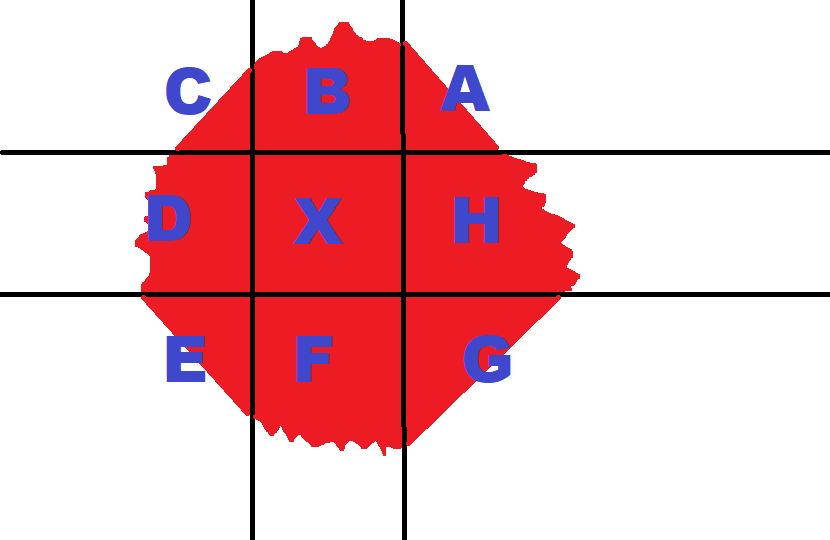
\includegraphics[width=8cm]{skogsbrand_bild.png}
\end{center}
\end{figure}

$\textbf{Delpoäng 4: }$ I den här testfallsgruppen är $M = 0$, $x_i, y_i < 100$, men $T$ kan vara hur stort som helst. Att simulera spridningen i upp till $10^9$ steg är helt uteslutet, vi måste hitta en annan strategi. En viktig observation är att "startområdet" är väldigt litet i jämförelse med $T$. Så efter att elden har spridit sig $T$ gånger kommer startområdet nästan se ut som en punkt, så det brinnande området borde nästan se ut som en Manhattancirkel. Låt oss anta att $T > 200$, om detta inte gäller så hinner vi simulera processen. Dela in planet i $9$ områden enligt bilden. Området $X$ är startrutan, dvs. alla punkter som uppfyller $0 \leq x,y \leq 99$. Eftersom $T > 200$ kommer hela startområdet vara brinnande, så det bidrar med $100\cdot 100$ till svaret. Låt oss se hur mycket de andra områdena bidrar. 
\begin{enumerate}

\item Område $A$ består av alla punkter som uppfyller $x,y \geq 100$. En punkt $(x,y)$ i område $A$ är brinnande om $|x-x'|+|y-y'| \leq T$ för någon av de givna punkterna $(x',y')$. Men $|x-x'|+|y-y'| = (x+y) - (x'+y')$ eftersom $x > x', y > y'$, så vi behöver bara bry oss om den givna punkt som har störst $x'+y'$. Området är alltså en kvartscirkel, och antalet punkter kan beräknas med en aritmetisk summa.

\item Område $B$ består av alla punkter som uppfyller $y \geq 100, 0 \leq x \leq 99$. Låt oss fixera en av dessa $x$-koordinater $x_0$, och se hur mycket $x_0$:s "stapel" bidrar med till svaret. En punkt $(x_0,y)$ i $B$ brinner om $|x_0-x'|+|y-y'| \leq T$ för någon given punkt $(x',y')$. Men $|x_0-x'| + |y-y'| = y + |x_0-x'|-y'$, så vi behöver bara hitta den givna punkt med minst $|x_0-x'|-y'$ för att hitta höjden på stapeln. Vi kan alltså kolla igenom alla $100$ värden på $x_0$, och hitta hur mycket var och en bidrar med.


\end{enumerate}
De andra områdena har samma utseende som $A$ eller $B$ och kan lösas på liknande sätt. \\
Här är en kul alternativ lösning som är svårare att komma på:

\begin{lemma}
    Låt $f(t)$ vara antalet punkter som brinner efter $t$ minuter. Låt oss anta att alla givna punkter är inom avstånd $W$ från varandra i $x$-led, och $H$ i $y$-led (i vårt fall är både $W,H = 100$). Då gäller det att 
    $$f(t+2)-2f(t+1)+f(t) = 4$$
    för alla $t > W+H$.
\end{lemma}
Notera att 
$$f(t+2)-2f(t+1)+f(t) = (f(t+2)-f(t+1))-(f(t+1)-f(t))$$
dvs. "ökningen av ökningen" eller accelerationen om man så vill. Man kan bevisa lemmat genom att kolla på bilden med de nio områdena igen. Område $B,D,F$ och $H$ kommer hela tiden öka med lika mycket, så de bidrar inget till accelerationen. Område $A,C,E,G$ däremot bidrar med $1$ var till accelerationen. \\
Problemet kan nu lösas genom att vi först simulerar i $201$ steg. Därefter beräknar vi $f(200)$ och $f(201)$. Låt $d$ vara $d = f(201)-f(200)$. Enligt lemmat blir nu $f(202) = f(201) + d + 4$, $f(203) = f(201) + d + 4 + d + 8$, osv. Mer allmänt får vi 
$$f(201+t) = f(201) + t\cdot d + 4\cdot (1+2+3+\dots+t) = f(201) + t\cdot d + 2t(t+1).$$
Så nu är det bara att stoppa in $t = T-201$ i formeln och så är vi klara. Svårt att komma på som sagt, men enklare att implementera. \\

$\textbf{Delpoäng 5: }$ Den här delpoängsnivån är samma som den förra fast det kan finnas nedhuggna träd. Lösningen är faktiskt ganska lik den förra också, vi kommer kunna reducera problemet till $M = 0$. Börja med att simulera processen i ungefär $500$ steg. Om de brinnande träden är helt instängda av nedhuggna träd så kommer det märkas, och vi kan bara skriva ut svaret. Annars så kommer elden att omringa alla nedhuggna träd vid det här laget. Vi kan alltså strunta i det inre av brandområdet där alla nedhuggna träd finns, eftersom inget nytt kommer hända där inne. Brandområdet kan nu betraktas som ett stort $(M = 0)$-testfall, och kan lösas med metoden från förra delpoängsnivån. Fast det här området är $1000 \times 1000$ och kan innehålla betydligt fler än $100$ brinnande punkter, så vi måste vara lite mer försiktiga. Ett sätt att hantera det på är att bara kolla på de brinnande punkter som är på kanten av brandområdet. Eftersom det är ca $4000$ såna punkter så borde lösningen till förra delpoängsnivån nu vara snabb nog. \\ Den alternativa lösningen till förra delpoängsnivån fungerar faktiskt här också, om vi simulerar lite fler steg och kollar om träden är instängda. \\

$\textbf{Delpoäng 6: }$ Den här testfallsgruppen kräver bara att $M = 0$. Den är samma som nivå $4$ fast koordinaterna kan vara stora, upp till $10^5$. Om $T \geq 2\cdot 10^5$ så kan vi faktiskt använda exakt samma lösning som i nivå $4$. Det som tar tid är att räkna ut hur mycket "staplarna" bidrar med, och eftersom det finns $4\cdot10^5$ staplar tar det ungefär $4\cdot 10^5\cdot n = 4\cdot 10^7$ steg, vilket är tillräckligt snabbt. Så det är när $T$ är "halvstort" som den här nivån kräver att vi gör något nytt. Det är att räkna ut antalet brinnande punkter i startområdet som är det svåra, för även om $T \leq 2\cdot 10^5$ så kommer vi kunna använda samma metoder som innan för att räkna brinnande punkter i de andra områdena. För att räkna antalet brinnande punkter i startområdet kan vi göra en så kallad svepning. Låt oss fixera en $x$-koordinat $x_0$. Vi vill räkna antalet brinnande punkter på formen $(x_0,y)$, där $0 \leq y < 10^5$. Varje given punkt $(x',y')$ kommer ge upphov till ett intervall på denna linje, som anger vilka träd som är inom avstånd $T$. Problemet blir nu att räkna ut antalet punkter som täcks av något av dessa $n$ intervall, och det kan lösas i $O(n\log(n))$ tid om man först sorterar intervallen. \\

$\textbf{Delpoäng 7: }$ Förut så simulerade vi för att reducera till $M = 0$. Men här blir det svårt eftersom det kan finnas nedhuggna träd väldigt långt från brinnande träd, så vi skulle behöva simulera alldeles för länge. I förra nivån kunde vi göra en svepning för halvstora $T$ och en enkel lösning för stora $T$, men en svepning verkar inte funka här eftersom elden kan slingra sig på konstiga sätt och inte ge upphov till intervall. Vi måste prova något nytt helt enkelt. \\
En sak vi inte har utnyttjat så mycket än är att antalet givna punkter bara är $200$. Vi skulle kunna använda koordinatkompression: att behandla de givna koordinaterna som "viktiga" och de andra som "likadana". Låt oss ta varje given punkt och dra $4$ räta linjer som går mitt emellan punkten och var och en av dess $4$ grannar, parallellt med $x$ och $y$-axlarna (se bild). Dessa linjer kommer dela in planet i ett antal rektanglar (ungefär $4\cdot (n+m)^2$ stycken). Det som är bra med dessa rektanglar är att elden når deras hörn först. Om elden skulle nå en rektangel på en sida innan den når något av hörnen så skulle det finnas intressanta koordinater längs med sidan, och då skulle inte rektangeln finnas. Så för varje rektangel vill vi räkna ut när elden först når var och en av dess fyra hörn. Det börjar likna ett kortaste vägen problem. Låt oss bygga en graf där alla hörn är noder. Dra kanter mellan par av noder som tillhör samma rektangel, där vikten är avståndet mellan punkterna. Dra också kanter mellan hörn som angränsar hörn i andra rektanglar. För att hantera nedhuggna träd behöver vi bara undvika att dra några kanter till dessa noder. Nu kan vi hitta kortaste vägen från de brinnande punkterna till alla hörn med Dijkstras algoritm, och så är vi nästan klara. Allt som återstår är att, givet när elden når alla fyra hörnen, räkna ut hur många punkter som brinner i varje rektangel. Det går att lösa det här matematiskt, men eftersom koordinaterna är så pass små hinner man faktiskt göra svepningar liknande dem i förra delpoängsnivån.

\begin{figure}[!h]
\begin{center}
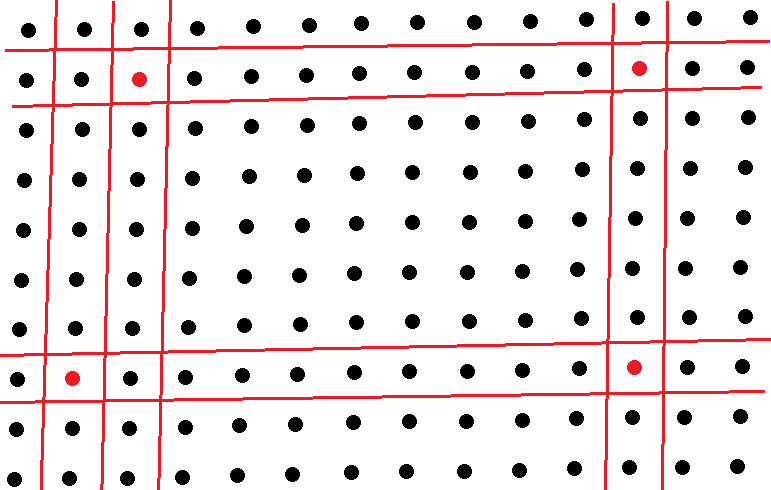
\includegraphics[width=8cm]{skogsbrand_2.png}
\end{center}
\end{figure}



\section{Lampknappar}
Vi börjar med att göra ett par observationer:
\begin{enumerate}
  \item Det finns ingen anledning att släcka lampor tidigt, utan man kan vänta till slutet med att göra det.
    Givet en lösning det att göra om det till en som väntar till slutet på följande sätt:
    \begin{itemize}
      \item simulera lösningen, men ignorera alla lampsläckningar
      \item gå motsatta vägen tillbaka till starten
      \item simulera lösningen igen, men släck nu varje rums lampa när du går ut ur rummet för sista gången
    \end{itemize}
    Eftersom varje lampa är tänd minst lika länge i den sista simuleringsprocessen kommer denna lösning fungera om den ursprungliga gör det,
    och vi noterar att vi först tänder alla lampor, och sen släcker dem.
  \item Problemet är symmetriskt: en lösning som går från rum $1$ till rum $N$ kan reverseras för att få en lösning som går från rum $N$ till rum $1$.
    En följd av detta är att rummen vi lyser upp i vår lösning kommer innehålla både en väg från nod $1$ till nod $N$, och en väg från nod $N$ till nod $1$.
  \item Det räcker att bara lysa upp dessa rum. Givet en väg från nod $1$ till nod $N$ och en väg från nod $N$ till nod $1$ kan vi göra följande:
    \begin{itemize}
      \item Gå från rum $1$ till rum $N$ och lys upp allt på vägen.
      \item Gå från rum $N$ till rum $1$ och lys upp allt på vägen.
      \item Gå från rum $1$ till rum $N$ igen.
      \item Ångra vandringen från rum $1$ till $N$ genom att gå motsatta hållet.
        När vi för sista gången går ut ur ett rum som inte är med i vandringen från rum $N$ till rum $1$, släck lampan i rummet.
      \item Ångra vandringen från rum $N$ till $1$ genom att gå motsatta hållet.
        När vi för sista gången går ut ur ett rum, släck lampan i rummet.
    \end{itemize}
    Det som får det här att funka är att vi alltid kan ångra en vandring genom att gå åt motsatt håll, utan att nånsin fastna i ett mörkt rum.
\end{enumerate}

\begin{figure}[!h]
\begin{center}
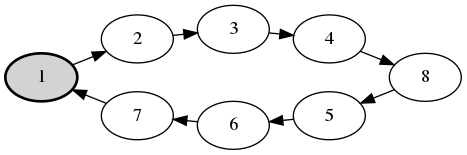
\includegraphics[width=5cm]{astep1.png}
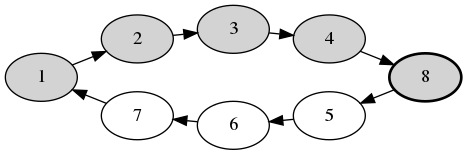
\includegraphics[width=5cm]{astep2.png}
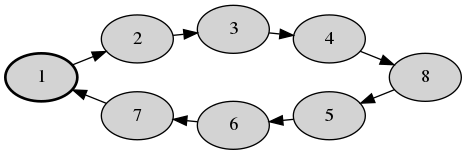
\includegraphics[width=5cm]{astep3.png}
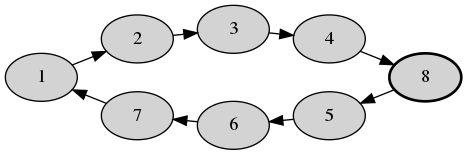
\includegraphics[width=5cm]{astep4.png}
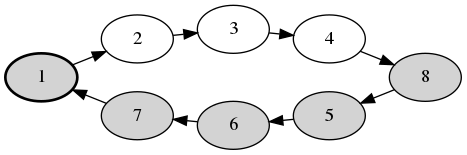
\includegraphics[width=5cm]{astep5.png}
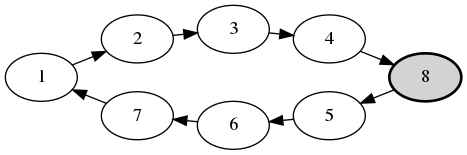
\includegraphics[width=5cm]{astep6.png}
  \caption{Illustration över hur lampornas tändande och släckande kan gå till, givet en väg från första till sista noden, och en väg från sista till första. Vägarna överlappar i det här fallet inte. En ifylld ruta betecknar ett upplyst rum, och tjock ram betyder att Ann just nu befinner sig i det rummet. Stegen visas vänster till höger, uppifrån ner.}
\end{center}
\end{figure}

\begin{figure}[!h]
\begin{center}
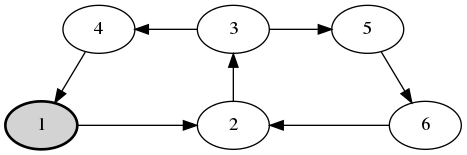
\includegraphics[width=5cm]{bstep1.png}
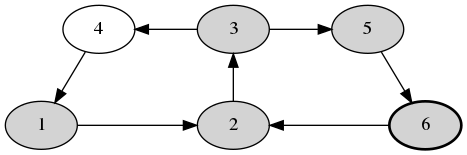
\includegraphics[width=5cm]{bstep2.png}
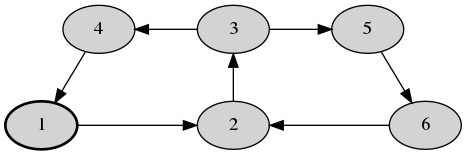
\includegraphics[width=5cm]{bstep3.png}
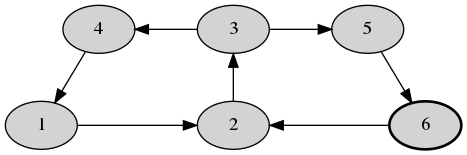
\includegraphics[width=5cm]{bstep4.png}
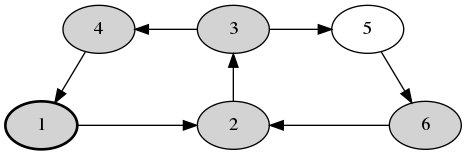
\includegraphics[width=5cm]{bstep5.png}
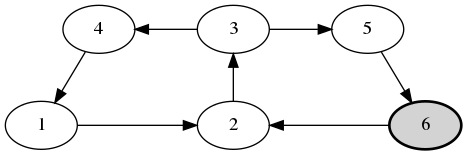
\includegraphics[width=5cm]{bstep6.png}
  \caption{Ett till exempel, med gemensamma noder på vägarna från start till slut och slut till start.}
\end{center}
\end{figure}

Det vi vill göra är alltså att hitta båda en väg från start till slut och en väg från slut till start, så att de tillsammans använder så få noder som möjligt.
I och med att dessa vägar interagerar med varandra skulle vi helst vilja konstruera dem tillsammans, en bit i taget.
Rimligtvis vill vi konstruera dem ``från vänster till höger'', med den ena vägen bakvänd, så att vi begränsar mängden interaktion --
om vi behöver minnas exakt hur vägarna vi konstruerat ser ut får vi lätt exponentiellt många tillstånd att hålla koll på, vilket inte hade fungerat.

Låt oss börja med att karaktärisera hur noderna de delar kan se ut, så att vi kan göra ovanstående mer konkret.
Tänk att det optimala svaret går från nod $1$ till nod $N$ genom noder $a_1, \dots, a_k$, och från nod $N$ till nod $1$ genom noder $b_1, \dots, b_k$.
På vilka sätt kan dessa vägar dela noder?
Rent intuitivt hade vi velat att de bara kan dela noder i motsatt ordning, så att ``vänster till höger'' blir något väldefinierat.

Låt oss tänka oss att nod $x$ och $y$ båda förekommer i både $a$ och $b$ i samma ordning.
I så fall kan vi ju minimera mängden noder i unionen av vägarna genom att låta vägen däremellan vara samma i $a$ och $b$.
I annat fall kommer noder att förekomma noder i omvänd ordning i $a$ och $b$, precis som vi hoppats.

Strukturen för en lösning ser därmed ut som i \ref{fig:lampstrukt} -- en massa gemensamma delsegment som kopplas ihop med vägar i olika riktningar.

\begin{figure}[!h]
\begin{center}
  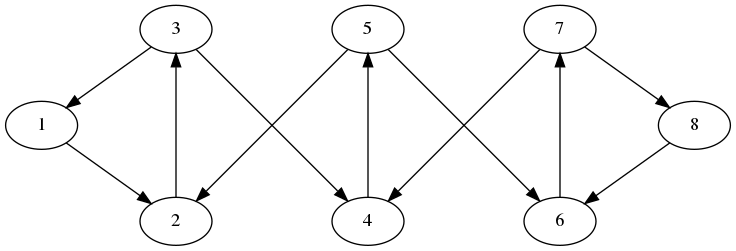
\includegraphics[width=10cm]{lampstrukt.png}
  \caption{Strukturen för en lösning. Varje kant kan ersättas av en väg med godtyckligt många noder.}
  \label{fig:lampstrukt}
\end{center}
\end{figure}

Vi kan nu återvända till vår tänkta lösning, där vi försöker konstruera de två vägarna från vänster till höger.
% Låt $E$ beteckna kanterna i graferna, och $E'$ kanterna i den omvända grafen (där alla kanter har bytt riktning).
Låt säga att vårt nuvarande tillstånd i konstruktionen av de två vägarna hela tiden är två noder $(u, v)$, rummen vi befinner oss i i framåt- och i bakåtvägarna.
Baserat på strukturen vi kommit fram till kan vi tänka oss att vi kan utföra tre olika möjliga operationer:
\begin{enumerate}
  \item Flytta $u$ framåt i grafen, till en granne.
  \item Flytta $v$ bakåt i grafen, till en granne i den reverserade grafen.
  \item Byt plats på $u$ och $v$.
\end{enumerate}

Den tredje operationen motsvarar att $u$ befinner sig i början av en delad väg och $v$ i slutet av den, och att $u$ rör sig framåt över vägen medan $v$ rör sig bakåt.

Fördelen med att vi konstruerar vägarna på sättet vi gör är att vi nu kan tilldela kostnader till de olika operationerna enbart baserat på vad $u$ och $v$ är, utan att behöva minnas hur vi flyttat oss tidigare.
Specifikt kan vi tänka att en operation av typ 1 kostar $0$ om $u$ flyttas till samma nod som $v$, annars $1$, och motsvarande för operationer av typ 2.
För operationer av typ 3 får vi en kostnad som motsvarar avståndet från nod $u$ till nod $v$ i grafen, minus $1$, i och med att noderna som är på vägen mellan $u$ och $v$ besöks exakt en gång vardera.
Se \ref{fig:lampexempel} för en illustration av hur lösningen för det andra exemplet kan beskrivas med hjälp av dessa operationer.

Givet dessa möjliga operationer och deras kostnader kan vi nu betrakta en ny graf med noder motsvarande tillstånd $(u, v)$, och kanter motsvarande operationer.
(För att beräkna kostnader för operationer av typ 3 kan vi först göra en BFS från alla noder, till kostnad $O(NE)$.)
I denna graf kan vi nu få ut vårt svar genom att göra en Dijkstra från tillstånd $(1, 1)$ till tillstånd $(N, N)$.

Antalet noder i grafen kommer att vara $O(N^2)$. Eftersom varje nods genomsnittliga antal utkanter är $2\cdot E/N + 1$ (varav $E/N$ för operationerna av typ 1 och 2, och $+ 1$ för operationen av typ 3), så kommer det totala antalet kanter att vara $O(N^2 \cdot E / N) = O(NE)$.
En Dijkstra tar därför $O(NE \log(NE))$ tid att genomföra, eller $O(NE)$ om vi utnyttjar att bara avstånd $1, 2, \dots, N-1$ är intressanta, och håller en kö för vardera av dem.
Addera till detta förberäkningen av alla kortaste avstånd som också är $O(NE)$, och vi får en total tidskomplexitet på $O(NE)$.

\begin{figure}[!h]
\begin{center}
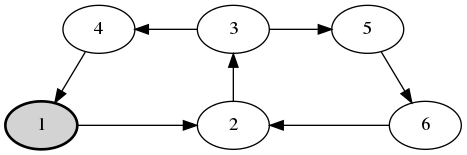
\includegraphics[width=5cm]{lampexempel1.png}
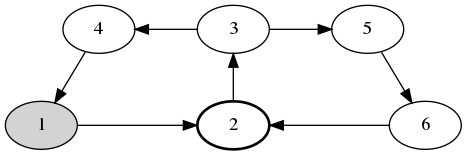
\includegraphics[width=5cm]{lampexempel2.png}
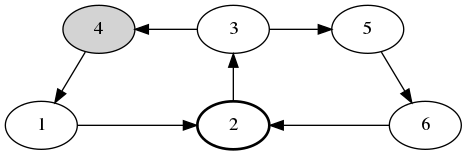
\includegraphics[width=5cm]{lampexempel3.png}
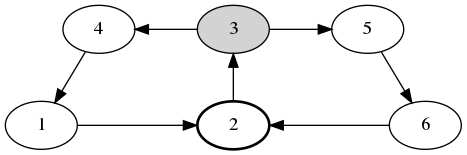
\includegraphics[width=5cm]{lampexempel4.png}
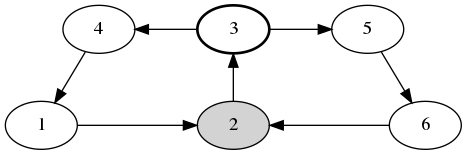
\includegraphics[width=5cm]{lampexempel5.png}
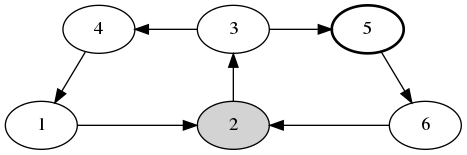
\includegraphics[width=5cm]{lampexempel6.png}
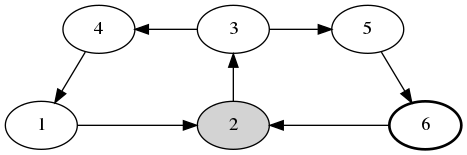
\includegraphics[width=5cm]{lampexempel7.png}
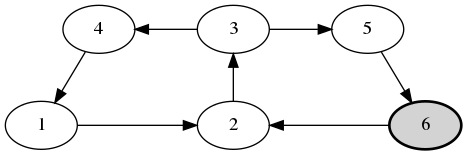
\includegraphics[width=5cm]{lampexempel8.png}
  \caption{Exempel av hur man med hjälp av operationer 1, 2 och 3 kan ta sig från tillstånd $(1,1)$ till tillstånd $(6,6)$ i grafen i det andra exemplet. $u$ betecknas med tjock ram, och $v$ med ifylld ruta.
  Stegen kostar i ordning 1, 1, 1, 0, 1, 1, 0, vilket ger en total kostnad på 5.}
  \label{fig:lampexempel}
\end{center}
\end{figure}


\end{document}
